\documentclass[11pt]{article}
\usepackage[T1]{fontenc}
\usepackage{mathptmx}
\usepackage[lmargin=3cm, rmargin=3cm, tmargin=2cm, bmargin=2cm]{geometry}
\usepackage{titlesec}
% Section headings: 14pt, bold
\titleformat{\section}
{\fontsize{14}{16}\selectfont\bfseries}
{\thesection}{1em}{}
% Subsection headings: 12pt, bold
\titleformat{\subsection}
{\fontsize{12}{14}\selectfont\bfseries}
{\thesubsection}{1em}{}
% Spacing: approximately two lines before and after
\titlespacing*{\section}
{0pt}{2\baselineskip}{2\baselineskip}
\titlespacing*{\subsection}
{0pt}{1\baselineskip}{1\baselineskip}

\usepackage{hyperref}
\usepackage{amsmath}
\usepackage{amssymb}
\usepackage{graphicx} % Required for inserting images
\graphicspath{{../graphs/}}
\usepackage{csquotes}
\usepackage[backend=biber]{biblatex}
\addbibresource{References.bib}
\usepackage{mathptmx}
\usepackage{float}
\usepackage{tabularx}
\usepackage{array}
\usepackage{algpseudocode}
\usepackage{algorithm}
\usepackage{todonotes}
\usepackage{tikz}
\usepackage{comment}

\newcolumntype{Y}{>{\raggedright\arraybackslash}X}
\renewcommand{\tabularxcolumn}[1]{m{#1}}

\title{A Comparative Analysis of Innovation Diffusion Models Based on Real-World Data}
\author{Noam Cisneros}
\date{2026/27}
\begin{document}
	
	\maketitle
	\thispagestyle{empty}
	\newpage
	\tableofcontents
	\thispagestyle{empty}
	\newpage
	
	\listoftodos
	
	\section{Introduction}
	Innovation diffusion is a field of mathematical modeling that has been extensively studied in the past, and many models have been created to model these types of processes.
	
	These different models describe the process of innovation diffusion on different levels of detail, with a greater or a lesser focus on the concrete decision process of the individual, and with different approaches to the general type of model used.
	
	This work aims to analyze the advantages and disadvantages these different models have for different uses of innovation diffusion modeling. The models analyzed are mainly described in the work of Ye and Zeno on the topic \autocite{Ye24}, in which the most important models are laid out. This paper in large part inspired this work. 
	
	I am personally fascinated by the topic of innovation diffusion due to its huge variety of mathematical approaches, as well as its direct relation to real life. I additionally find it interesting to see how well the predictions of certain innovation diffusion Models are quite directly visible in everyday life; whenever a piece of information is spreading in a group of people, even when it only consists of a few individuals, one can quite easily observe all processes described by the mathematical model and how they actually influence decision process. In general, the persistence of mathematical patterns in human behavior is very interesting in my opinion, as they reveal how strongly collective human behavior follows mathematical patterns, which we oftentimes do not realize.
	
	This strong occurrence of innovation diffusion theory is also the main reason for the relevance of this field of mathematics. Due to the theory of innovation diffusion being a quite generic theory, the applications of it range from fields like Sociology to economy, politics and many others.
	
	In the following, I will first give a short theoretical introduction to some mathematical methods used to model innovation diffusion. Then, I will describe the three models of innovation diffusion that I will compare in this work, namely the Bass Diffusion model, a modified version of the Linear Threshold Model and a Game-Theoretic Model, and explain in detail how each of the models approaches the topic of innovation diffusion. Pseudocode for the implementation of the models as well as the GitHub repository with the Python code can be found in appendix \ref{app:Scripts}. After that, I will fit each of the models to a real dataset, and will compare how well they manage to describe the innovation process and how consistently they can be used.
	Finally, I will answer the following research question:
	\textit{To what extent are the Bass Diffusion Model, the Linear Threshold Model, and the Game-Theoretic Model suitable for modelling real-world innovation diffusion, considering their computational efficiency, interpretability, and predictive capabilities?} 
	
	\section{Theoretical Basis}
	\subsection{Networks} \label{sec:NetworksBasis}
	A common assumption in innovation diffusion models is that an individual’s adoption decision depends on its social environment. Both the Linear Threshold Model and the Game-Theoretic Model incorporate this assumption through a network of interacting agents. Formally, such a network is represented by a graph consisting of a set of vertices (or nodes), $\mathcal{V}$, and a set of edges, $\mathcal{E}$, where each edge connects a start vertex to an end vertex. The network I am using is a so-called \textit{directed graph}, meaning that it is not necessarily the case that if node $A$ is connected to node $B$, node $B$ is also connected to node $A$. For each node $i \in \mathcal{V}$, the set of neighbouring nodes is denoted by $\mathcal{N}_i$, which contains all nodes with which individual $i$ can interact. The number of neighbours of node $i$ is given by $d_i = |\mathcal{N}_i|$ and is referred to as the \textit{degree} of node $i$ in the network. This notation follows the convention used by Ye and Zino \autocite{Ye24}. An example of how such a graph might look like can be seen in figure \ref{fig:network} Each node has a time-dependent state, denoted $\mathbf{x}_i(t)$. This value encodes wether or not the node has accepted the innovation or not, with $\mathbf{x}_i$ being equal to 1 when the innovation is adopted by agent $i$, and 0 otherwise. The fraction of agents that have adopted the innovation at time $t$ is then equal to
	
	$$
	|\mathcal{V}|\underset{\mathcal{i \in \mathcal{V}}}{\sum}\mathbf{x}_i(t)
	$$
	\\
	and will be denoted by $\zeta(t)$.
	
	\begin{figure}[H]
		\centering
		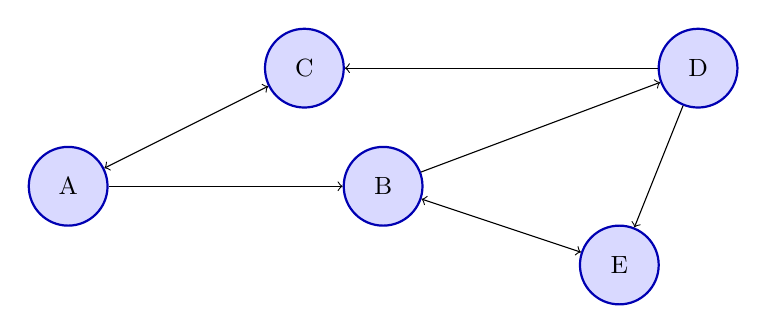
\begin{tikzpicture}[
			node/.style={
				circle,
				draw=blue!70!black,
				fill=blue!15,
				thick,
				minimum size=10mm,
				font=\small
			},
			edge/.style={
				thick,
				draw=gray!80
			}
			]
			% Define nodes
			\node[node] (A) at (1.0, 0.0)  {A};
			\node[node] (B) at (5.0, 0.0)  {B};
			\node[node] (C) at (4.0, 1.5)  {C};
			\node[node] (D) at (9.0, 1.5)  {D};
			\node[node] (E) at (8.0, -1.0) {E};
			% Define connections
			\draw[<->] (A) -- (C);
			\draw[->]  (A) -- (B);
			\draw[<->] (E) -- (B);
			\draw[->]  (D) -- (E);
			\draw[->]  (B) -- (D);
			\draw[->]  (D) -- (C);
		\end{tikzpicture}
		\caption{An example of a small directed network, with the following properties: $\mathcal{V}=\{ A,B,C,D,E \}, \quad \mathcal{E} = \{ (A,C), (C,A), (A,B), (B,E), (E,B), (B,D), (D,E), (D, C) \}$}
		\label{fig:network}
	\end{figure}
	
	\subsection{Differential Equations}
	When describing systems that change dynamically over time, Differential Equations (DEs) are oftentimes a helpful mathematical tool, as they can predict how a system will change in an infinitesimally small time-step, given only the state of the system in the current time-step. 
	The Bass Diffusion Model is based on a Differential Equation (DE). A DE is an equation that relates a function to its own derivatives. When only the first derivative of the function and the function itself appears in the DE, it is called a \textit{first-order Differential Equation}. The Bass Diffusion Model is such a first-order Differential Equation \autocite{Bass69}. Since time is the only independent variable in the Bass Diffusion Model, the equation describing it is a so-called Ordinary Differential Equation (ODE).
	
	DEs generally do not have solutions that can be expressed in closed form. If this is the case, their solutions can only be evaluated numerically with a given initial condition using algorithms such as the Runge-Kutta Method \autocite{Runge}. While the Bass Diffusion model does have a closed form solution (see section \ref{sec:BassModel} for the derivation), I implemented it with a numerical algorithm for simplicity.
	
	\subsection{Game Theory - payoff matrices} \label{sec:payoff}
	An important concept in Game Theory and mathematical modeling in general are so-called payoff matrices. A payoff matrix encodes advantages and disadvantages of making certain decisions in a two-player coordination game with respect to the decision the opposing player takes. Such a payoff matrix can be written as follows:
	$$\mathbf{P} = 
	\begin{pmatrix} 
		a & b \\
		c & d
	\end{pmatrix}$$
	where $a$ is the reward for choosing to play $1$ against an opponent who also chose $1$, while $c$ is the reward for playing $1$ against an opponent who played $0$. similarly, $b$ is the reward for playing $0$ against $1$, and d is the reward for playing $0$ against $0$. 
	
	It should be noted that the matrix given above is not the most general notion of a two-player game that exists; rather, it encodes payoffs in a so-called \textit{symmetric game}. a symmetric game is one where both players receive the same payoff for choosing the same actions against the same opponent action. a game that is not symmetric consists of two payoff matrices, one for each player, where the payoffs are not equal in general. Since such a model is unnecessarily complex for the purpose of modeling innovation diffusion, all games considered in this work will be assumed to be symmetric.
	\todo{write more about coordination games}
	
	\section{The three Diffusion Models}
	The three models I will compare in this work are the Bass Diffusion Model, which has a differential equation as its basis, The Linear Threshold model, which is based on a network of individuals with differently strong tendencies to adopt the innovation, and a version of a Game-Theoretic model, which is centered around the idea of two-player coordination games and following emerging trends.
	
	\subsection{The Bass Diffusion Model} \label{sec:BassModel}
	The Bass Diffusion model is one of the first concrete mathematical models of innovation diffusion. It is defined by the ordinary differential equation
	
	\begin{equation} \label{eqn:Bass}
		\frac{d\zeta}{dt} = (1-\zeta) (p+q\zeta)
	\end{equation}
	
	where $\zeta(t)$ is the fraction of adopters at time t, and $p$ and $q$ are positive, real-valued parameters \autocite{Bass69}.
	
	This differential equation can be solved via seperation of variables as follows:
	
	$$
	\frac{d\zeta}{(1-\zeta)(p+q\zeta)} = dt.
	$$
	
	Integrating both sides yields
	\begin{equation} \label{eqn:Integral}
		\int \frac{d\zeta}{(1-\zeta)(p+q\zeta)} = t.
	\end{equation}
	
	The Integral on the left-hand side of the equation can be rewritten by using partial fraction decomposition on the integrand:
	
	\begin{equation*}
		\begin{split}
			\frac{1}{(1-\zeta)(p+q\zeta)} &= \frac{A}{1-\zeta}+ \frac{B}{p+q\zeta} \\
			1 &= A(p+q\zeta) + B(1-\zeta) \\
			1 &= Ap + Aq\zeta + B - B\zeta.
		\end{split}
	\end{equation*}
	
	
	By comparing coefficients, one gets the two equations
	
	$$ Aq - B = 0 $$
	
	and
	
	$$ Ap + B = 1. $$
	
	Solving this system of linear equations, $A$ and $B$ evaluate to
	
	\begin{equation*}
		\begin{split}
			A &= \frac{1}{p+q} \\
			B &= \frac{q}{p+q}.
		\end{split}
	\end{equation*}
	
	Equation \ref{eqn:Integral} can now be rewritten as follows:
	
	$$
	\int\frac{1}{(p+q)(1-\zeta)} + \frac{q}{(p+q)(p+q\zeta)} =t.
	$$
	
	factoring out the term $\frac{1}{p+q}$ and using the linearity of the integral to split it into the sum of two integrals gives
	
	$$
	\frac{1}{p+q} \left( \int \frac{d\zeta}{1-\zeta} + q\int \frac{d\zeta}{p+q\zeta} \right) = t.
	$$
	
	Both integrals can be solved using a simple $u$-substitution. The equation can then be solved for t:
	
	\begin{equation*}
		\begin{split}
			\frac{1}{p+q}[\ln(p+q\zeta) - \ln(1-\zeta)] &= t +C \\
			\ln \left( \frac{p+q\zeta}{1-\zeta} \right) &= (p+q)t + C \\
			\frac{p+q\zeta}{1-\zeta} &= e^{(p+q)t}\cdot C \\
			p+q\zeta &= e^{(p+q)t}\cdot C(1-\zeta) \\
			p+q\zeta &= e^{(p+q)t}C - e^{(p+q)t}C\zeta \\
			p &= e^{(p+q)t}C - e^{(p+q)t}C\zeta - q\zeta \\
			p &= e^{(p+q)t}C - \zeta \left( e^{(p+q)t}C +q \right) \\
		\end{split}
	\end{equation*}
	
	The final expression for $\zeta(t)$ then becomes
	
	\begin{equation}
		\boxed{\zeta(t) = \frac{e^{(p+q)t}C-p}{e^{(p+q)t}C+q}}.
	\end{equation}
	\todo{C in terms of y(0)}
	
	This function produces an S-shaped curve \todo{not accurate}, with the parameters $p$ and $q$ determining how exactly the curve is shaped. Roughly speaking, $p$ controls the steepness of the curve at its beginning, while $q$ controls the steepness at the end \todo{fix this}. Figures \ref{fig:bassfixedp} and \ref{fig:bassfixedq} visualise the effect of the parameters on the diffusion curve.
	
	\begin{figure}[H]
		\centering
		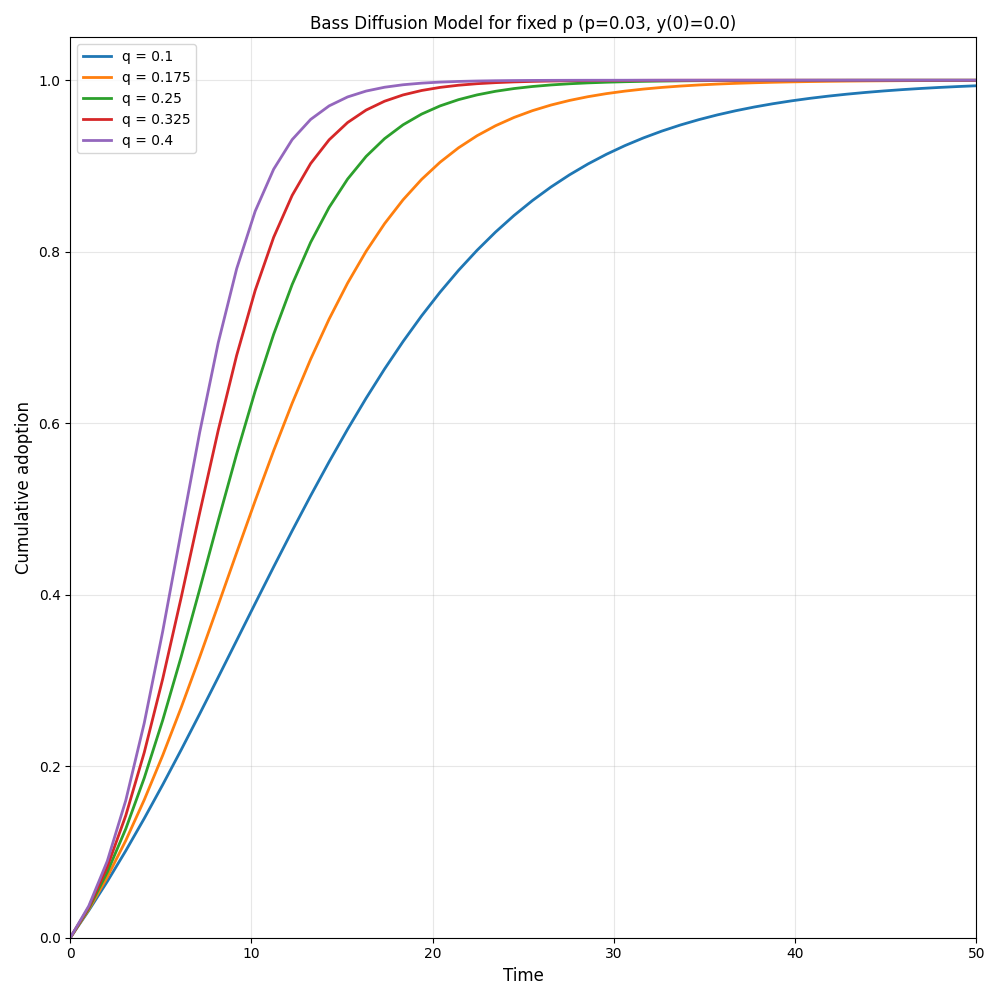
\includegraphics[width=1\linewidth]{Bass_fixed_p}
		\caption{Bass Diffusion Model with fixed $p$.}
		\label{fig:bassfixedp}
	\end{figure}
	
	\begin{figure}[H]
		\centering
		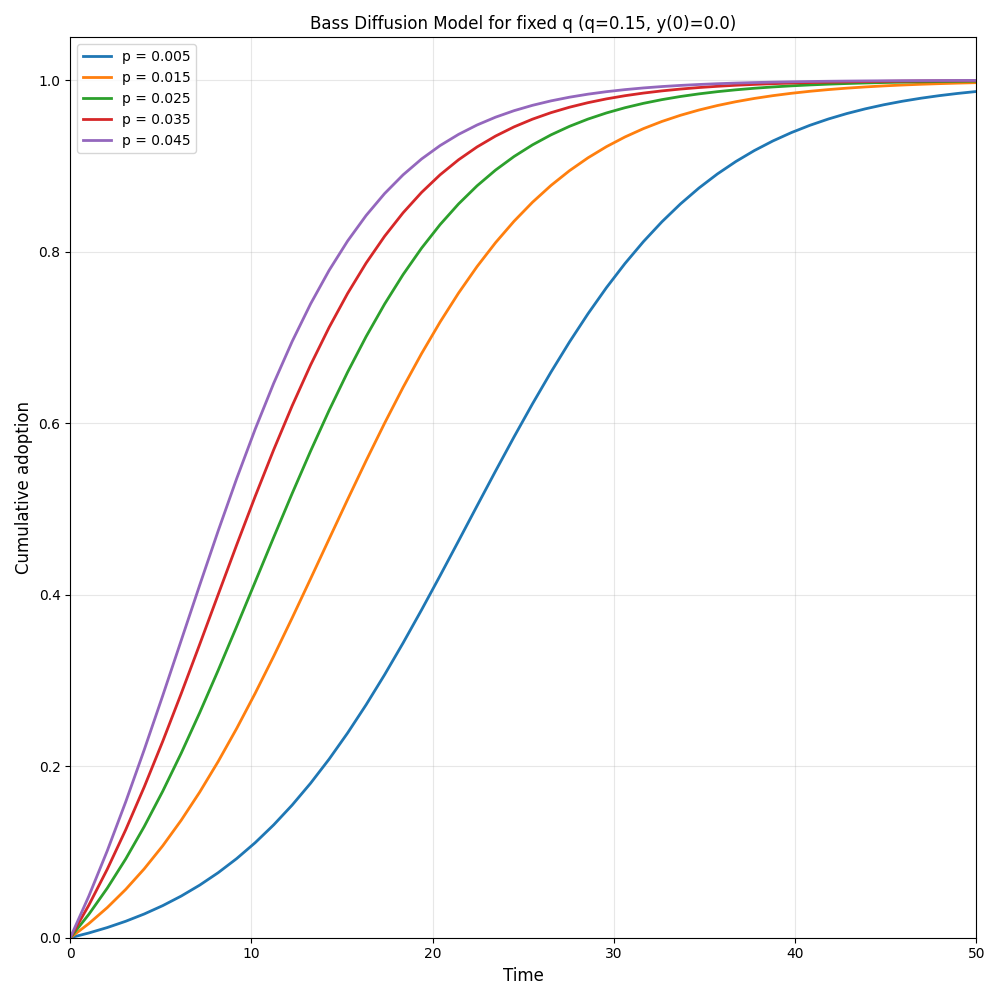
\includegraphics[width=1\linewidth]{Bass_fixed_q}
		\caption{Bass Diffusion Model with fixed $q$.}
		\label{fig:bassfixedq}
	\end{figure}
	
	\subsection{The Linear Threshold Model} \label{sec:LinearThreshold}
	The Linear Threshold Model, henceforth referred to as LTM, initially proposed by Mark Granovetter in 1978 \autocite{Granovetter78}, is a diffusion model that is based on a network similar to the one described in section \ref{sec:NetworksBasis}. Each node has a set of neighbours $\mathcal{N}_i$, and a threshold $\theta_i$ that lies in the interval $[0,1]$. The threshold describes how easily the individual accepts the innovation; in practice, it is the fraction of neighbours of the node that need to adopt the innovation in order for the node itself to adopt it as well \autocite{Granovetter78}. Thus, the update rule for the LTM can be formalized as follows:
	
	$$\mathbf{x}_i(t+1) = 
	\begin{cases}
		1, & \text{if \quad} \frac{1}{\lvert \mathcal{N}_i \rvert} \underset{j \in \mathcal{N}_i}{\sum} \mathbf{x}_j(t) \geqslant \theta_i\\
		0, & \text{if \quad} \frac{1}{\lvert \mathcal{N}_i \rvert} \underset{j \in \mathcal{N}_i}{\sum} \mathbf{x}_j(t) < \theta_i.\\
	\end{cases}
	$$
	\\
	Recall from section \ref{sec:NetworksBasis} that $\mathbf{x}_i(t)$ stands for the state of node $i$ at time $t$, where a state of 0 means that the agent has not adopted the innovation, while a state of 1 means that the agent has adopted the innovation. The sums in the update rule are equal to the average of the states of all neighbours of the node. When a node has accepted the innovation, it sets it threshold to 0, meaning that it cannot revert to the status quo.
	
	This is the most basic Linear Threshold Model, described by Granovetter \autocite{Granovetter78}. I did a few minor modifications to the model, in order to make it more practical for the specific purpose of fitting the curve to a dataset, as described in section \ref{sec:dataFitting}.
	
	The main way in which my Model differs from the one described by Granovetter \autocite{Granovetter78}is that it does not update all nodes at every time-step. Instead, I defined a parameter $p \in [0; 1]$ called the \textit{update probability}, which is the probability that a node will update at a certain time-step. The reason for this is to mirror the fact that people do not realistically re-evaluate their decisions as often as the model assumes. It also makes the model's predictions more consistent and makes it easier and more intuitive to control how many time-steps the diffusion process should last.
	
	In practice, it is not possible to assign the thresholds to each node manually, so they have to be sampled randomly. This is why in my model the thresholds are sampled from a normal distribution with a mean $\mu$ and a standard deviation $\sigma$ \todo{explain truncated normal distribution}. One problem with this is that a normal distribution allows outputs that are negative or greater than 1, while $\theta_i$ has to lie between 0 and 1. I fixed this issue by forcing the node to re-evaluate its threshold in the initialization phase of the simulation until a value between 0 and 1 is reached. This means that the final distribution used for the threshold evaluation is actually a so-called \textit{truncated normal distribution}. One important consequence of this is that the parameters $\mu$ and $\sigma$ are the mean and standard deviation of the original gaussian, \textit{not} of the actual threshold distribution.
	
	The specific implementation I used works as follows:
	
	first, the initial state of the population is determined by a set \textit{seed fraction}; this parameter determines which fraction of the nodes adopt the innovation at time-step 0. All seed nodes will have a threshold of 0, meaning that it is impossible for them to revert to the status quo. Every node that is not marked as a seed node will start with the state 0, which means it will have the status quo.
	
	After the set of seed nodes have been set, each node selects a set of neighbours by choosing a set of nodes randomly from the network. A node cannot chose itself as its own neighbour. Since it is possible that one node $A$ has node $B$ as its neighbour, while $B$ does not have $A$ as its neighbour, this produces a directed network as described in section \ref{sec:NetworksBasis}. After the node has selected its set of neighbour nodes, it picks a threshold from the normal distribution as described above.
	\\
	In total, the network has six parameters:
	
	\begin{table}[H]
		\centering
		\begin{tabularx}{\textwidth}{|>{\centering\arraybackslash}m{1.3cm}||l|X|}
			\hline
			Symbol & Variable name in the code & meaning \\
			\hline
			$d$ & \texttt{num\textunderscore neighbours} & The number of neighbours of each node, or the degree of the network \\
			\hline
			$|\mathcal{V}|$ & \texttt{num\textunderscore agents} & The number of agents in the network \\
			\hline
			$\zeta(t=0)$ & \texttt{seed\textunderscore frac} & The fraction of all nodes acting as "seed nodes" \\
			\hline
			$\mu$ & \texttt{mean} & The mean value of the threshold distribution \\
			\hline
			$\sigma$ & \texttt{stdev} & The standard deviation of the threshold distribution \\
			\hline
			$p$ & \texttt{update\textunderscore prob} & The probability that a node will update at any given time-step. This parameter is the same for every node. \\ \hline
		\end{tabularx}
		\caption{The parameters of the Linear threshold model}
		\label{tab:parameters-LTM}
	\end{table}
	
	The most important parameters here are $\mu$ and $\sigma$, as they determine how easily the population adopts the innovation.
	
	After the network has been initialized, the simulation process begins. In each step, the model loops through each node in $\mathcal{V}$, and adjusts its state according to the update rule described at the beginning of the section. It is important to note that the node does not immediately change its state; if it were to do so, the order in which the nodes were updated would affect the outcome of the model. Instead, every updated state is stored in an array together with the index of the node it belongs to. After every node in the network has written its new state to the array, all nodes are actually updated using the data from the array. This leads to the nodes effectively updating at the same time.
	
	For the details of the models implementation, see Appendix \ref{app:Scripts}.
	
	It should be noted that this implementation of the LTM is quite a simple one; possible generalizations and improvements include assigning weight to each edge in the network based on how socially compatible two nodes are (a comparable idea has been investigated by Axelrod \autocite{Axelrod97}), to introduce more than two possible states for the agents to chose from, and many more.
	
	\subsection{Game-Theoretic Model} \label{sec:GTM}
	Game Theory offers a good framework for innovation diffusion models, since its focus is on decision processes. When these processes are applied to individuals in a network that can decide between two states, 0 and 1, where 0 denotes adoption of the status quo and 1 denotes an adoption of the innovation, a diffusion process can be observed.
	
	As proposed by Zino et al. \autocite{Zino23}, a time-varying network was used in the simulation. This means that each node re-evaluated its neighbours in each time-step of the simulation, which reduces the effect of the network structure on the curve of the diffusion process by approximating a randomly mixing population. Like for the LTM, I also used an update probability for this model.
	
	The agents in the Game-Theoretic model can follow two update rules. Which one they follow is picked at random by each node at every time-step. The idea for this is taken from Zino et al. \autocite{Zino23}.
	
	The first of the two update rules is based on a payoff matrix (see section \ref{sec:payoff}, while the second update rule is based on following emerging trends. The probability that the second update rule is chosen by a node is called the \textit{trend-sensitivity} of the network, and will be denoted $s$. 
	
	
	
	\subsubsection{Update Rule 1: Coordination Games}
	When following the first update rule, the individuals will engage in a two-player coordination game with their neighbours. The node will decide whether or not to adopt the other node's state according to a payoff matrix.
	
	Recall the definition of the generic payoff matrix introduced in section \ref{sec:payoff}:
	
	$$\mathbf{P}=\begin{pmatrix} 
		a & b \\
		c & d
	\end{pmatrix}$$
	The total payoff for node $i$ received for choosing action $k$ (notated here as $\pi_i(x_i = k)$) is then defined simply as the sum of the payoffs received by the all of the neighbours of node $i$:
	
	\begin{equation} \label{eq:payoffs}
		\begin{split}
			\pi_i(\mathbf{x}_i = 0) &= \sum_{j \in \mathcal{N}_i}  x_j b + (1 - x_j) d \\
			\pi_i(x_i = 1) &= \sum_{j \in \mathcal{N}_i}  x_j a + (1 - x_j) c
		\end{split}
	\end{equation}
	
	Assuming that the individuals always chose the option which returns the greatest payoff, the state of individual $i$ at the next time-step will result from the following best-response update rule:
	
	$$\mathbf{x}_i(t+1) = \underset{k \in \{0; 1\}}{\arg \max}(\pi_i(x_i = k)).$$
	
	This means that the Agent will always simply choose its next state such that the payoff $\pi_i$ received for the choice is maximised.
	
	The payoff matrix I used for my analysis was proposed by Zino et al. \autocite{Zino23}. It simplifies the model by writing the payoff matrix as
	
	$$ \mathbf{P} = \begin{pmatrix}
		1 + \alpha & 0 \\
		0          & 1
	\end{pmatrix},$$
	
	Where the parameter $\alpha$, called the \textit{relative advantage} of the innovation, rewards the action of accepting the innovation. The reason for this is that the payoff for choosing to follow neighbours who adopted the innovation is increased relative to the payoff received for following neighbours who follow the status quo by the factor $1+\alpha$. This can be thought of as "increasing the influence" of the neighbours who accepted the innovation on the total payoff in equation \ref{eq:payoffs}. \todo{explain exactly what effect alpha has on the update rule}
	
	\subsubsection{Update Rule 2: Trends}
	Informally, he idea of this update rule is that an individual will adopt the innovation if it notices that the fraction of adopters has increased in the previous time-steps.
	
	Concretely, individual $i$ updates its state according to the following rule:
	
	$$ \mathbf{x}_i(t+1) = 
	\begin{cases}
		1 \text{ if } \zeta(t) - \zeta(t-1) > 0 \\
		0 \text{ if } \zeta(t) - \zeta(t-1) < 0 \\
		\mathbf{x}_i(t) \text{ else}
	\end{cases}.
	$$
	
	This update rule was also proposed by Zino et al. \autocite{Zino23}.
	\\
	\\
	In total, the Game-Theoretic Model has the following parameters:
	
	\begin{table}[H]
		\centering
		\begin{tabularx}{\textwidth}{|>{\centering\arraybackslash}m{1.3cm}||l|X|}
			\hline
			Symbol & Variable name in the code & meaning \\
			\hline
			$d$ & \texttt{num\textunderscore neighbours} & The number of neighbours of each node, or the degree of the network \\
			\hline
			$|\mathcal{V}|$ & \texttt{num\textunderscore agents} & The number of agents in the network \\
			\hline
			$\zeta(t=0)$ & \texttt{seed\textunderscore frac} & The fraction of all nodes acting as "seed nodes" \\
			\hline
			$\alpha$ & \texttt{alpha} & The relative advantage of the innovation. Increases the payoff of playing 1 against an opponent who also played 1. \\
			\hline
			$s$ & \texttt{trend\textunderscore sensitivity} & The probability that a node will update based on trends rather than payoff. \\
			\hline
			$p$ & \texttt{update\textunderscore prob} & The probability that a node will update at any given time-step. This parameter is the same for every node. \\ \hline
		\end{tabularx}
		\caption{The parameters of the Game-Theoretic model}
		\label{tab:parameters-GTM}
	\end{table}
	
	\section{Data Fitting} \label{sec:dataFitting}
	
	\subsection{The Dataset}
	The dataset I used to fit the models to comes from a collection of datasets about the spread of new technologies in the US, supplied by "Our World in Data" \autocite{datasetDiffusion}. The used the dataset about the fraction of US households owning a refrigerator, labelled \texttt{Refrigerator} in the dataset collection. The dataset contains data from 1920 to 2017 \todo{check}, but I only used the data from 1925 to 1980 \todo{check}, since a plateau is already reached roughly around 1960. It should be noted that every node in the simulation of the LTM and Game-Theoretic Model will represent a single household, not an individual.
	There are several reasons for why I chose this specific dataset. First of all, the data shows a very clear adoption curve, with the adopter fraction starting at 0.01 in 1925 and reaching a plateau at 0.99. Another reason for why this dataset is well-suited for this analysis since the decision whether or not to buy a refrigerator is actually made by the households themselves in most cases, and social influences can be assumed to contribute to this decision.
	
	\subsection{The Optimisation Algorithm}
	Every one of the three models has a certain set of parameters, or inputs, that determine the prediction it makes. When fitting a specific model to the dataset, the idea is to find the optimal values for these three parameters such that the model's output aligns with the dataset as closely as possible. To find these optimal parameters, I used the \texttt{differential\textunderscore evolution} optimisation algorithm from the Python package \texttt{scipy}, with a mean-squared error function.
	
	What this means is that the model is initialized with random parameters, and given an error score, which rates how well the model predicted the dataset. This score is evaluated as follows:
	
	$$ E = \frac{1}{n}\sum_{i=0}^n (y_i - \hat{y}_i)^2, $$
	
	where $n$ is the length of the dataset, $y_i$ is the models prediction for $\zeta$ at the $i$th time-step, and $\hat{y}_i$ is the actual fraction from the dataset. After this error is evaluated, the \texttt{differential\textunderscore evolution} algorithm then "mutates" the parameters in a specific way in order to find parameters that produce a lower error, in a similar way to how genetic mutation leads to species adopting to their environment in nature \autocite{DifferentialEvolution}.
	
	The \texttt{differential\textunderscore evolution} method takes the following parameters:
	
	\begin{itemize}
		\item \texttt{bounds}: the minimum and maximum values for each of the parameters that are being optimised.I determined the bounds by manually testing the model with different values and seeing in which range the parameters should roughly lie.
		\item \texttt{maxiter}: the maximum number of iterations the algorithm is allowed to run before having to return a result. This value was always set to 1000.
		\item \texttt{tol}: the \textit{tolerance} of the algorithm. The smaller this number is, the closer the algorithm will try to get to the dataset. This value was always set to 0.001. \todo{WRONG: explain tol}
	\end{itemize} 
	
	\subsection{The Bass Diffusion Model}
	The Bass Diffusion model was the easiest model to optimise, since it only has two parameters and runs extremely quickly. The optimisation for the Bass model was run with the bounds
	
	\begin{table}[H]
		\centering
		\begin{tabular}{|c|c|c|}
			\hline
			parameter & minimum & maximum \\ \hline
			$p$       & 0.0001  & 1       \\ \hline
			$q$       & 0.0001  & 1       \\ \hline
		\end{tabular}
	\end{table}
	
	\begin{figure}[H]
		\centering
		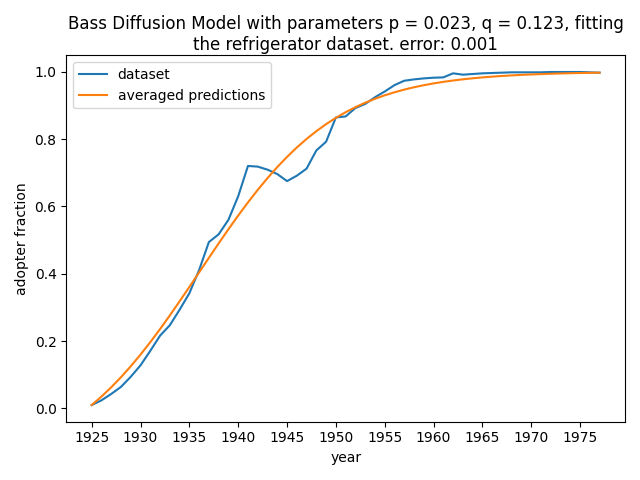
\includegraphics[width=0.8\textwidth]{Bass_fit}
		\caption{Output of the Bass Diffusion Model fitting the dataset.}
		\label{fig:pred-Bass}
	\end{figure}
	
	\subsection{The Linear Threshold Model} \label{LTM-dataFitting}
	For the data fitting, the thresholds were again sampled from a normal distribution that is the same for all nodes, as described in Section \ref{sec:LinearThreshold}. The number of Agents was fixed to 500, since this is the largest network which my computer could simulate reasonably fast. After manually experimenting with the parameter $d$, I found that a value of 10 produced good results. There were three parameters that I optimized, namely the standard deviation $\sigma$ and the mean $\mu$ of the distribution, as well as the update probability $p$. I used the following ranges for the optimisation algorithm:
	
	\begin{table}[H]
		\centering
		\begin{tabular}{|c|c|c|}
			\hline
			parameter & minimum & maximum \\ \hline
			$\mu$     & 0.001   & 0.8     \\ \hline
			$\sigma$  & 0.001   & 0.3     \\ \hline
			$p$       & 0.001   & 0.6     \\ \hline
		\end{tabular}
	\end{table}
	
	\subsection{The Game-Theoretic Model} \label{sec:fitting-GTM}
	
	The Game-Theoretic model was considerably harder to optimise than the Linear Threshold Model, mainly because the relative advantage $\alpha$ can take any value from 0 to infinity. This means that I had to find the approximate upper bound manually through a trial-and-error process. I eventually arrived at the conclusion that an $\alpha$ value between 0 and 2 would produce a consistent result with the correct values for $p$ and $s$. This led me to the following bounds:
	
	\begin{table}[H]
		\centering
		\begin{tabular}{|c|c|c|}
			\hline
			parameter & minimum  & maximum \\ \hline
			$\alpha$  & 0.0      & 2.0     \\ \hline
			$s$       & 0.1      & 0.3     \\ \hline
			$p$       & 0.001    & 0.4     \\ \hline
		\end{tabular}
	\end{table}
		
	\section{Results}
	This section concerns itself with the general characteristics of each model. The models will be investigated mainly with respect to how easy or practical they are to use, which errors or complications they produce, and for which populations they produce a viable 
	result.
	
	\subsection{The Bass Diffusion Model}
	The optimal parameters for the Bass Diffusion model are
	
	\begin{table}[H]
		\centering
		\begin{tabular}{|c|c|}
			\hline
			$p$ & $q$     \\ \hline
			0.023 & 0.123 \\ \hline
		\end{tabular}
		\caption{Optimal parameters for the Bass Diffusion Model}
		\label{tab:paramsBass}
	\end{table}
	
	
	
	\subsection{The Linear Threshold Model} \label{LTM_results}
	Optimising the LTM to the dataset yielded a minimum of the MSE score with the following parameters: 
	
	\begin{table}[H]
		\centering
		\begin{tabular}{|c|c|c|}
			\hline
			$p$ & $\mu$ & $\sigma$ \\ \hline
			0.226 & 0.085  & 0.054 \\ \hline
		\end{tabular}
		\caption{Optimal parameters for the LTM}
		\label{tab:paramsLTM}
	\end{table}
	
	The low value of $\mu$ means that the individuals are required to accept the innovation quite easily in order for the model to produce a curve that fits the dataset closely.
	
	It should be noted that the average MSE error is the average of the errors for each run. The same is true for the Game-Theoretic Model in the next section.
	
	One big issue I encountered when running the LTM with these parameters is that the results vary quite strongly. This was, however, fixed by introducing the update probability $p$ described in section \ref{sec:LinearThreshold}. Still, randomness is part of the model, so I ran the model 50 times with the same parameters and used the average of all the resulting curves to get the final value for the average error of the model. This process is visualised in figure \ref{fig:pred-LTM}, where the gray curves are the actual runs of the model, while the orange line is the average.
	
	After fixing these issues, I managed to get the LTM to predict the real dataset quite closely, with an average Score of about 0.004. Figure \ref{fig:pred-LTM} shows the final fit of the LTM.
	
	\begin{figure}[H]
		\centering
		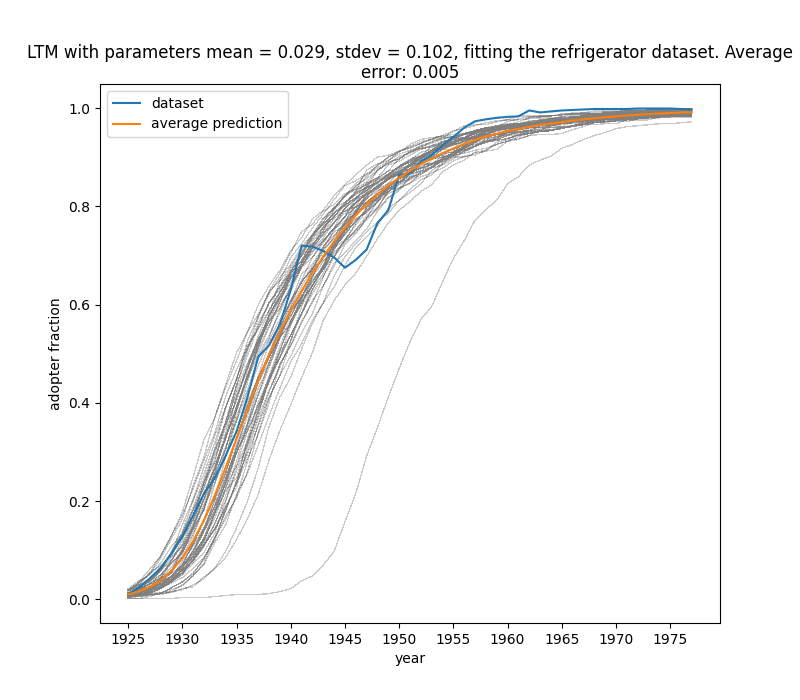
\includegraphics[width=0.8\textwidth]{LTM_fit}
		\caption{Averaged outputs of the LTM fitting the dataset.}
		\label{fig:pred-LTM}
	\end{figure}
	
	
	\subsection{The Game-Theoretic Model}
	After running the Game-Theoretic Model through the same optimisation algorithm, I found the following set of ideal parameters:
	
	\begin{table}[H]
		\centering
		\begin{tabular}{|c|c|c|}
			\hline
			$p$ & $\alpha$ & $s$   \\ \hline
			0.111 & 1.305  & 0.348 \\ \hline
		\end{tabular}
		\caption{Optimal parameters for the Game-Theoretic Model}
		\label{tab:paramsGTM}
	\end{table}
	\todo{what is the interpretation of these optimal parameters?}
	
	\begin{figure}[H]
		\centering
		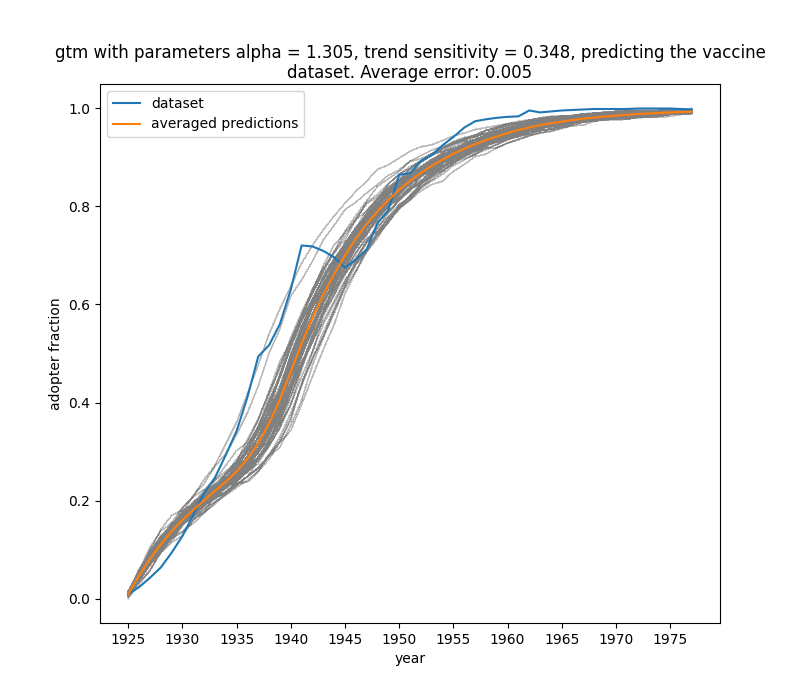
\includegraphics[width=1\linewidth]{../graphs/GTM_fit}
		\caption{Averaged outputs of the Game-Theoretic Model predicting the \texttt{BCG Vaccine\textunderscore Share of Population\textunderscore PK} dataset.}
		\label{fig:pred-GTM}
	\end{figure}
	
	\section{Comparison}
	The three models will be compared with respect to the following aspects:
	\begin{itemize}
		\item \textit{Fitting accuracy:} How well could each model fit the data?
		\item \textit{Computational efficiency:} How efficient are the models computationally?
		\item \textit{Realism:} How realistic are the assumption of each model?
		\item \textit{Interpretability:} How well can the parameters of the models be interpreted?
		\item \textit{Modelling capabilities:} Which adoption processes can the models describe?
	\end{itemize}
	
	\section{Discussion}
	\subsection{Limits}
	While the dataset used for data fitting in section \ref{sec:dataFitting} does model a general diffusion process, there are some factors contributing to the curve of the data that the models do not account for. The models assume that the decision to buy a refrigerator is only influenced by the social environment of the household in question, while factors such as the affordability of refrigerators are ignored.
	
	\section{Outlook}
	\todo[inline]{Summary, final fazit, etc.}
	
	\newpage
	\appendix
	\section{Appendix: symbols and naming conventions}
	The following table contains important symbols and their meanings.
	\begin{table}[H]
		\centering
		\begin{tabularx}{\textwidth}{|p{1cm}|X|}
			\hline
			Symbol & Meaning \\
			\hline
			$\zeta(t)$ & The relative fraction of adopters at time $t$\\ \hline
			$N(t)$ & The absolute number of adopters at time $t$ \\ \hline
			$p$    & The probability of a node to update its state at any given time-step \\ \hline
			
			\multicolumn{2}{|c|}{Linear Threshold Model} \\ \hline
			$\mathcal{V}$ & Set of nodes in the network \\ \hline
			$\mathcal{E}$ & Set of Edges in the network \\ \hline
			$\mathcal{N}_i$ & Set of neighbours of Node $i$ \\ \hline
			$d_i$ & The degree of node $i$, or $|\mathcal{N}_i|$ \\ \hline
			
			\multicolumn{2}{|c|}{Game-Theoretic Model} \\ \hline
			$\mathbf{P}$ & Payoff matrix \\ \hline
			$\alpha$ & Relative advantage of the innovation \\ \hline
			
		\end{tabularx}
		\caption{naming conventions}
		\label{tab:namings}
	\end{table} \todo{complete the table}
	
	\section{Appendix: Python scripts} \label{app:Scripts}
	\subsection{Linear Threshold model}
	The Pseudocode for the implementation of the LTM found on GitHub looks as follows:
	
	\begin{algorithm}[H]
		\caption{The Linear Threshold Model} \label{alg:LTM}
		\begin{algorithmic}
			\For{$i$ in $\mathcal{V}$}
			\State $\theta_i \gets$ random value sampled from $\mathcal{N}(\mu, \sigma)$ such that $0<\theta_i<1$
			\State $\mathbf{x}_i \gets$ 1 with probability $p$ = seed fraction, 0 otherwise
			\State $\mathcal{N}_i \gets$ select a random set of neighbours from $\mathcal{V}$
			\EndFor
			\State
			\While{executed iterations $<$ maximum iterations}
			\For{$i$ in $\mathcal{V}$}
			\If{a random value is below $p$}
			\State evaluate $\mathbf{x}_i(t+1)$ based on the update rule
			\If {$\mathbf(x)_i(t+1) = 1$}
				\State Set $\theta_i$ to 0
			\EndIf
			\State store the result in the state array
			\Else
			\State store the current state $\mathbf{x}_i(t)$ in the state array
			\EndIf
			\EndFor
			\For{$i$ in $\mathcal{V}$}
			\State update the state $\mathbf{x}_i$ using the corresponding value in the state array
			\EndFor
			\EndWhile
		\end{algorithmic}
	\end{algorithm}
	
	\todo{pseudocode for GTM}
	
	\newpage
	\todo{insert URLs for the references}
	\printbibliography
\end{document}
